\documentclass[12pt]{article}

\usepackage[T1]{fontenc}
\usepackage[utf8]{inputenc}
\usepackage[russian]{babel}
\usepackage{xcolor}
\usepackage{minted}
\usepackage{graphicx}
\usepackage{float}
\usepackage{caption}
\usepackage[margin=1.5cm]{geometry}

\addto\captionsrussian{\renewcommand{\figurename}{Рисунок}}
\renewcommand{\listingscaption}{Фрагмент программы}

\setlength{\abovecaptionskip}{3pt plus 0pt minus 0pt}
\setlength{\belowcaptionskip}{0pt plus 0pt minus 0pt}

\captionsetup[listing]{position=bottom,skip=-10pt,font=small}
\captionsetup[figure]{position=bottom,skip=12pt,font=small}

\newminted{python}
{
    frame=lines,
    framesep=2mm,
    baselinestretch=1.2,
    bgcolor=darkgray,
    fontsize=\footnotesize,
    python3,
    style=monokai,
    rulecolor=white
}

\title{Разбор задач конкурса "Звезды Кассиопеи"}
\date{20.05.2021}
\author{Надобных Дмитрий, Пугач Сергей, Чечеватов Роман}

\begin{document}
    \pagenumbering{gobble}
    \maketitle
    \pagenumbering{arabic}
    \newpage
    \raggedright

    \section{Ручные задачи}

    \subsection{MP5}
    \paragraph{}
    Эта задача засчитывалась как решенная после перехода по ссылке.
    Ничего сложного.

    \subsection{Автостоп}
    \paragraph{}
    Как сказано в условии, ответом на данную задачу является ответ на Главный вопрос жизни, вселенной и всего такого.
    Вопрос этот был задан английским писателем Дугласом Адамсом в книге \verb|"The Hitchhiker’s Guide to the Galaxy"|,
    русским читателям известной как \verb|"Автостопом по галактике"|.
    \paragraph{}
    Участники, читавшие этот роман могут спокойно ответить \verb|42| и получить баллы,
    остальным придется скопировать вопрос в Гугл и получить ответ в первом же результате.
    \paragraph{Ответ:}
    \verb|42|

    \subsection{Язык программирования}
	\paragraph{}
    Для решения этой задачи участникам необходимо было изучить HTML-код страницы задачи.
	Для этого можно воспользоваться встроенными в браузер инструментами разработчика,
	или скачать страницу и открыть в текстовом редакторе.
	\paragraph{}
	Независимо от выбранного способа, ответ находился в комментарии рядом с формой ввода ответа.
    \begin{figure}[H]
        \centering
        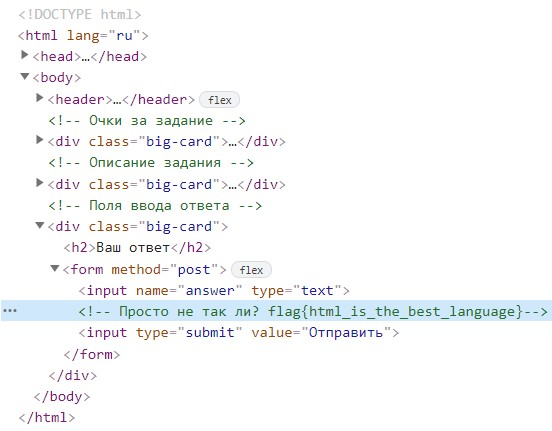
\includegraphics[width=12cm]{task45}
        \label{fig:task45}
        \caption{HTML-код страницы задачи}
    \end{figure}
    \paragraph{Ответ:}
    \verb|flag{html_is_the_best_language}|

    \subsection{Фотосессия}
	\paragraph{}
    В данной задаче участникам давался для анализа JPG-файл с картинкой.
	Однако, такие файлы зачастую содержат в себе не только данные изображения, но и дополнительную информацию.
	Например, дату съемки, модель камеры, имя автора.
	И среди этой дополнительной информации и был спрятан флаг.
    \paragraph{Ответ:}
    \verb|flag{haha_you_thought_it_will_be_ccv}|

    \subsection{PI}
	\paragraph{}
    Здесь участников просили ввести число Пи с некоторой точностью:
	строго заданное число знаков после запятой, не больше и не меньше.
	Достаточно точное число Пи можно взять на Википедии или, для пользователей Windows 10, Калькуляторе.
    \paragraph{}
    Отгадать необходимую точность можно с помощью метода проб и ошибок, или просто написав бота.
    \paragraph{Ответ:}
    \verb|3.14159265358979323846264338327|

    \subsection{Задача, которую невозможно решить}
	\paragraph{}
    Вопреки сказанному в названии задачи, ее возможно решить.
	Наличие решения этой задачи показывает,
	как внимательно участники прочитали инструкцию по работе с тестирующей системой.
	Ведь именно в разделе \verb|Мануал|, в подразделе \verb|Обработка персональных данных|,
	совершенно не к месту находилось предложение
    ''Однако, для решения задачи, которую невозможно решить, вам нужно всего лишь отправить название конкурса''.
	Остается лишь найти правильное с точностью до символа название.
    \paragraph{Ответ:}
    \verb|Звёзды Кассиопеи|

    \subsection{Двадцать пятый кадр}
	\paragraph{}
    В данной задаче участникам предлагался для анализа файл с видео.
	И хотя в метаданных на этот раз флага не было, там можно было обнаружить частоту кадров видео: 120~кадров в секунду.
	Это значит, что на экранах с частотой обновления 60~Гц и менее
	(а таких на момент проведения конкурсов подавляющее большинство)
	немалая часть кадров просто не будет отображаться.
	Но зачем же авторы дали видео с таким большим числом кадров, зная, что часть из них не будет показана?
	Неужели они хотели что-то там спрятать?
	Да.
	Смотрим видео покадрово и на 817~кадре замечаем серый текст на сером фоне.
    \begin{figure}[H]
        \centering
        
\includegraphics[width=10cm]{task30}
        \label{fig:task30}
        \caption{Один из кадров видео}
    \end{figure}
    \paragraph{Ответ:}
    \verb|flag{you_have_great_eyes}|

    \subsection{Eglishman}
	\paragraph{}
    В очередной раз отправляемся в Гугл (Яндекс, Bing, DuckDuckGo, Рамблер, Поиск~Маил.Ру,~\ldots)
	чтобы узнать, как сервер может узнать местоположение/страну/язык пользователя и узнаем, два основных способа:
	по~IP и по предпочитаемому языку пользователя.
    \paragraph{}
	Методом проб и ошибок, испробовав все платные и бесплатные VPN-сервера узнаем,
	что в данной задаче IP ничего не значит.
    \paragraph{}
	Остается вариант с языком.
	Браузер внутри запроса отправляет информацию о предпочитаемом языке веб-страниц.
	В настройках браузера выставляем предпочтение на английский, отправляем что угодно в качестве ответа и получаем баллы.

    \subsection{1C}
	\paragraph{}
    В следующей задаче на анализ содержимого файла участникам был дан файл Excel.
	Изучив свойства файла или создав новый лист, можно обнаружить,
	что кроме видимого листа с многозначащим названием \verb|Лист1| в книге есть еще два: \verb|Лист2| и \verb|Лист3|.
	В Microsoft Office Excel жмем ПКМ по списку листов, \verb|Показать...|, \verb|Лист2|.
	Изучаем содержимое ранее скрытого листа рядом с красивой картинкой аэродинамических характеристик коровы
	обнаруживаем флаг.
    \begin{figure}[H]
        \centering
        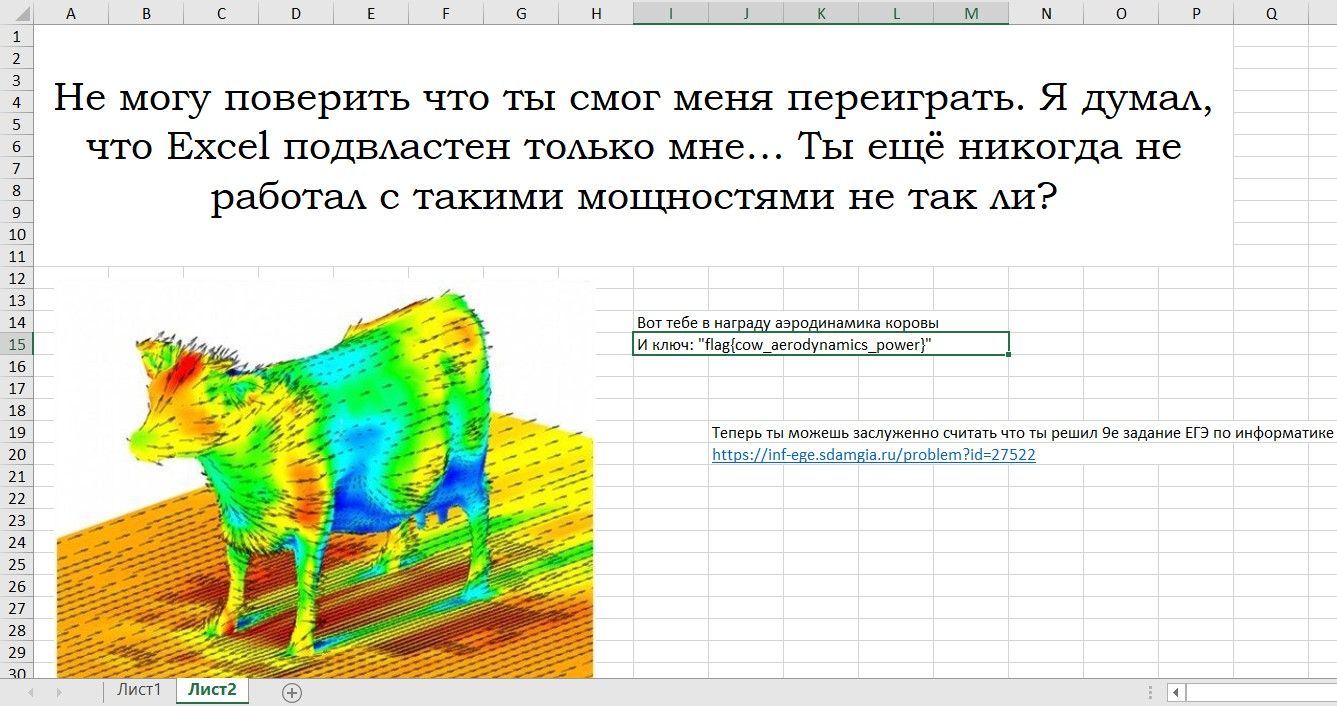
\includegraphics[width=12cm]{task11}
        \label{fig:task11}
        \caption{Скрытый лист с ответом}
    \end{figure}
    \paragraph{Ответ:}
    \verb|flag{cow_aerodynamics_power}|

    \subsection{Машина времени}
	\paragraph{}
    Снова скачиваем приложенный файл.
	Распаковываем архив, наряду с привычными, но ничем не примечательными файлами обнаруживаем папку \verb|.git|.
	Или не обнаруживаем, если у вас не включено отображение скрытых файлов.
	В таком случае, включаем, потому что без него заниматься поиском скрытой информации весьма непросто.
    \paragraph{}
	В любом случае, закинув название папки в Гугл получаем понимание, что авторы дали вам Git-репозиторий.
	Git - одна из систем контроля версий, то есть позволяет отслеживать и сохранять изменения файлов,
	откатываться к предыдущей версии.
    \paragraph{}
	Скачиваем Git, устанавливаем.
	Делаем коммит с помощью \verb|git commit -a|, видим, что после последнего коммита (сохранения) файлы изменялись.
	Откатываемся к предыдущему коммиту \verb|git checkout a23d2c7|,
    смотрим содержимое когда-то бывшего удаленным файла, находим флаг.
    \paragraph{Ответ:}
    \verb|flag{wayback_machine_master}|

    \subsection{Восьмая симфония Чайковского}
    \paragraph{}
    Любой уважающий себя третьеклассник знает, что самым лучшим форматом файла для хранения изображения является \verb|mp3|.
    К пятому классу дети узнают, что это всё же не лучшее место для хранения картинок, но всё ещё подходящее.
    Я говорю об обложке альбома - картинке, которую можно вложить в файл \verb|mp3|.
    При этом она не обязана действительно быть обложкой альбома, там может быть всё что угодно.
    Хотя, чтобы не вызывать много подозрений, мы нашли какую-то похожую картиночку, на которой написали флаг.
    Да, писали светлым по светлому, но никто не обещал, что будет просто.
    \begin{figure}[H]
        \centering
        
\includegraphics[width=7cm]{task51}
        \label{fig:task51}
        \caption{Картинка из файла 51.mp3}
    \end{figure}
    \paragraph{Ответ:}
    \verb|flag{fade_in_music}|

    \subsection{Я - Гуль}
    \paragraph{}
    В данной задаче участникам предлагалось использовать обученную заранее нейронную сеть для выполнения задачи распознавания и анализа образов.
    С использованием такой нейронной сети можно с лёгкостью понять, какое математическое выражение находится в приложенном к заданию файле.
    Допускается также использование этой нейронной сети для вычисления значения выражения.
    \paragraph{}
    Если считать нейронной сетью множество связанных нейронов, то головной мозг человека можно назвать нейронной сетью.
    Я не биохим.
    \paragraph{}
    А задачу мы предлагаем решать вручную.
    Серьёзно: чтобы получить образцы всех цифр, нужно правильно заслать не менее 8 раз.
    А после такого уже и до полного решения недалеко.

    \subsection{Spectre}
    \paragraph{}
    Название задачи говорит об амплитудно-частотном анализе.
    Это явно не просто так, в отличие от остальных задач.
    Заметим, что спектрограмма позволяет выполнить неплохой амплитудно-частотный анализ "на глаз".
    \paragraph{}
    Открываем файл в чем-нибудь, что умеет строить спектрограмму, например \verb|Audacity|.
    Далее задача решается методом пристального вглядывания в эту спектрограмму.
    \begin{figure}[H]
        \centering
        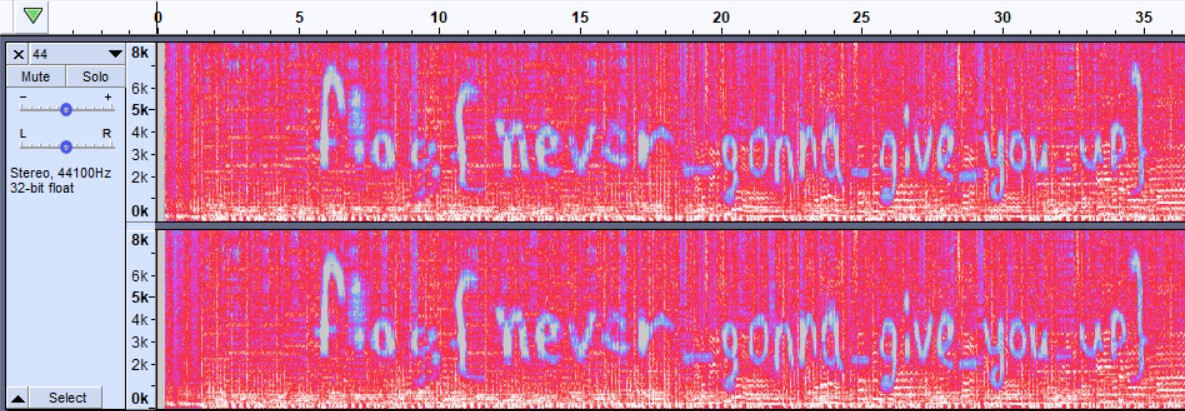
\includegraphics[width=\linewidth]{task44}
        \label{fig:task44}
        \caption{Фрагмент спектрограммы}
    \end{figure}
    \paragraph{Ответ:}
    \verb|flag{never_gonna_give_you_up}|

    \subsection{Пленочный фотоаппарат}
    \paragraph{}
    Скоро напишем разбор
    % TODO
    \paragraph{}
    Ответ: \verb|flag{that_was_a_good_2.3BTC}|

    \subsection{Пленочный фотоаппарат 2}
    \paragraph{}
    Скоро напишем разбор
    % TODO
    \paragraph{}
    Ответ: \verb|flag{that_was_my_last_money}|

    \newpage

    \section{Задачи на использование ботов}
	\paragraph{}
    Для начала рассмторим общую для всех ботов часть: работу с сетью.
	Мы использовали для написания ботов \verb|Python 3| и библиотеку \verb|requests|.
	Ничто не мешало вам использовать другие варианты,
	а незнание любого из них компенсируется длиной конкурса и доступностью все того же Гугла.
	\paragraph{}
    Импортируем библиотеку и задаем константы:
    \begin{listing}[H]
        \begin{pythoncode}
# -*- coding: utf-8 -*- # Волшебное слово, чтобы использовать кириллицу
import requests # Импортируем requests

login = 'login' # Сохраняем логин и токен
token = '23847634320439b65adafb7e3fefff802b1cde0a1b2977c3fe299a6dd111e4ce'
host = 'https://fetefot763.eu.pythonanywhere.com/'
        \end{pythoncode}
        \caption{Импортируем requests}
        \label{lst:import_requests}
    \end{listing}
    \paragraph{}
    Теперь нужно разобраться, как браузер отправляет запросы на сайт.
    Открываем панель разработчика и изучаем (смотри рисунок~\ref{fig:browser1}).
    \begin{figure}[H]
        \centering
        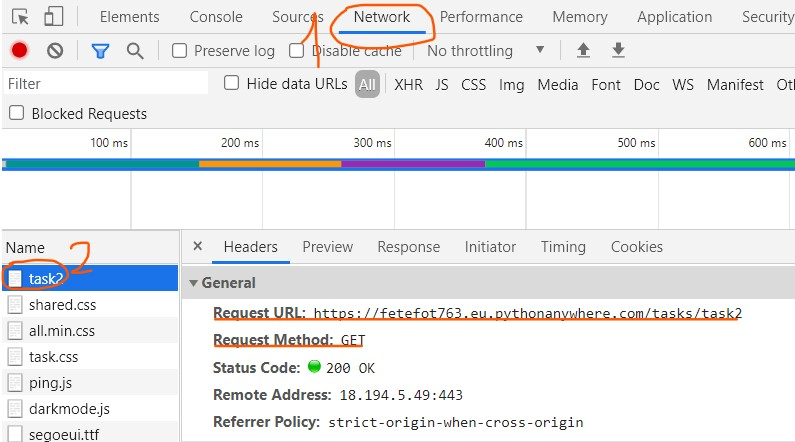
\includegraphics[width=15cm]{BrowserNetworkAnalysis0}
        \caption{Изучение процесса получения страницы браузером.}
        \label{fig:browser1}
    \end{figure}
    \paragraph{}
    Видим, что браузер отправляет GET-запрос на страницу задачи.
    Продолжаем изучение, проматываем вниз (смотри~рисунок~\ref{fig:browser2}).

    \begin{figure}[H]
        \centering
        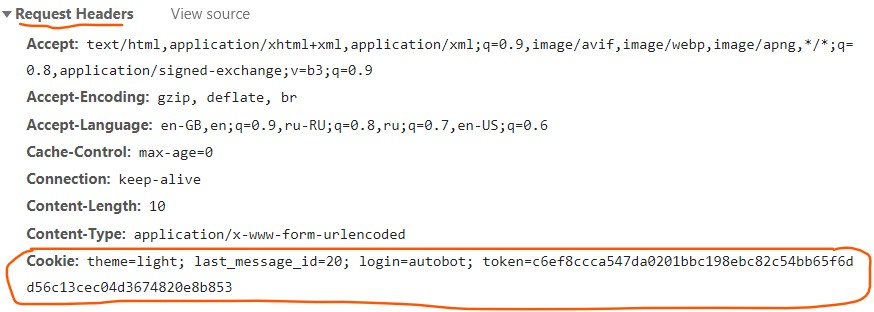
\includegraphics[width=15cm]{BrowserNetworkAnalysis2}
        \caption{Изучение отправляемых браузером cookie-файлов.}
        \label{fig:browser2}
    \end{figure}
    \paragraph{}
    Теперь видим, что браузер отправляет cookie-файлы, чтобы получить страницу.
    Почитав в мануале обнаруживаем, что для работы необходимо только две печеньки: \verb|login| и \verb|token|.
    Их значения сохраняем к себе и используем дальше.
    \paragraph{}
    Используя полученные знания мы можем написать функцию получения задачи.
    Функция - это обособленный фрагмент кода, выполняющий узкую задачу.
    \paragraph{}
    Для задач, где в приложении дан текст, мы можем получить этот текст прямо со страницы задачи:

    \begin{listing}[H]
        \begin{pythoncode}
# Для текстовых задач (на примере задачи №1 - Водолей)
def get_data():                                   # Объявляем функцию
    text = requests.get(                          # Отправляем запрос
        host + 'tasks/task1',                     # На страницу задачи
        cookies={'login': login, "token": token}  # С cookies авторизации
    ).text                                        # И сохраняем текст ответа в переменную text
    return text                                   # Возвращаем text
        \end{pythoncode}
        \caption{Получение содержимого текстовой задачи}
        \label{lst:get_data_text}
    \end{listing}
    \paragraph{}
    Заметим, что функция \verb|get_data| возвращает нам весь HTML-код страницы.
    Нам же нужно только приложение к заданию.
    Приложения всегда находятся в блоке с \verb|id="task_data"| и не содержат блоков внутри.
    Пользуясь этим, создадим новую функцию для извлечения этого приложения:

    \begin{listing}[H]
        \begin{pythoncode}
def get_text_from_data(data):
    marker_beg = '<div id="task-data">'
    marker_end = '</div>'
    ind_beg = data.rfind(marker_beg) + len(marker_beg)  # Индекс начала содержимого блока в строке
    ind_end = data[ind_beg:].find(marker_end)           # Индекс конца содержимого блока в строке
    text = data[ind_beg:ind_beg + ind_end]              # Сохраняем содержимое блока в переменную
    return text                                         # Возвращаем text
        \end{pythoncode}
        \caption{Получение текста задачи из содержимого}
        \label{lst:get_text_from_data}
    \end{listing}

    Следует четко понимать, какую задачу вы решаете и какие функции из приложенных вам следует использовать.
    Так, функция получения текста задачи вернет мусор, если текста в задаче не окажется.
    А что произойдет с вашей программой при попадании внутрь мусора никому не известно.
    \paragraph{}
    Если же в приложении дана ссылка на файл, то его нужно скачать.
    Тогда функция может ничего не возвращать: результат запроса уже сохранен в файл и будет прочитан из него.

    \begin{listing}[H]
        \begin{pythoncode}
# Для файловых задач (на примере задачи №2 - WinRar 3000)
def get_data():                                          # Объявляем функцию
    requests.get(                                        # Отправляем запрос
        host + 'tasks/task2',                            # На страницу задачи
        cookies={'login': login, "token": token}         # С cookies авторизации
    )
    with open('2.zip', 'wb') as file:                    # Создаем и открываем файл 2.zip для записи
        file.write(                                      # Записываем в файл
            requests.get(                                # Отправляем запрос
                host + f'task-generated-content/2/task2_{team_id}.zip', # За файлом
                cookies={'login': login, "token": token} # С cookies авторизации
            ).content                                    # Записываем в файл ответ на запрос
        )
        \end{pythoncode}
        \caption{Получение приложенного файла задачи}
        \label{lst:get_data_file}
    \end{listing}
    \paragraph{}
    Теперь проанализируем отправку браузером нашего решения задачи.
    Напишем что-нибудь в поле ответа и нажмем кнопку отправки.
    Посмотрим, что же нам показывает браузер в уже знакомой панели (смотри~рисунок~\ref{fig:browser3}).

    \begin{figure}[H]
        \centering
        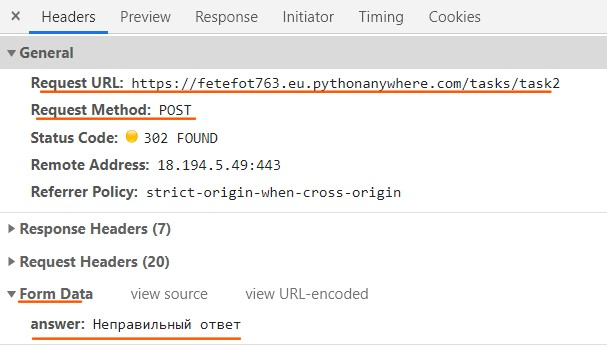
\includegraphics[width=15cm]{BrowserNetworkAnalysis3}
        \caption{Изучение отправки браузером ответа на задачу.}
        \label{fig:browser3}
    \end{figure}
    \paragraph{}
    Видим, что браузер отправляет запрос все на ту же страницу, но уже POST-запрос.
    В запрос браузер включает \verb|данные формы|, содержащие поле \verb|answer| со значением,
    которое мы только что вписали в поле ввода ответа.
    Как всегда, cookie браузер тоже отправляет.
    \paragraph{}
    Напишем функцию отправки ответа в данных формы:

    \begin{listing}[H]
        \begin{pythoncode}
def send_data(data):                              # Объявляем функцию
    requests.post(                                # Отправляем запрос
        host + f'tasks/task{task_id}',            # На страницу задачи
        data={'answer': data},                    # С данными формы
        cookies={'login': login, "token": token}  # И cookies авторизации
    )
        \end{pythoncode}
        \caption{Отправка ответа на задачу}
        \label{lst:send_data}
    \end{listing}
    \paragraph{}
    На этом работа с сетью завершается.
    Остается только в правильном порядке вызывать наши функции:

    \begin{listing}[H]
        \begin{pythoncode}
# Для текстовых задач
if __name__ == '__main__':                        # Если запущен именно этот файл
    while True:                                   # Вечный цикл
        txt = get_text_from_data(get_data())      # Получаем текст задачи
        res = solve(txt)                          # Решаем задачу и сохраняем ответ
        send_data(res)                            # Отправляем ответ
        \end{pythoncode}
        \caption{Основной цикл программы решения текстовой задачи}
        \label{lst:mainloop_text}
    \end{listing}

    \begin{listing}[H]
        \begin{pythoncode}
# Для файловых задач
if __name__ == '__main__':                        # Если запущен именно этот файл
    while True:                                   # Вечный цикл
        get_data()                                # Получаем данные
        res = solve()                             # Решаем задачу и сохраняем ответ
        send_data(solve())                        # Отправляем ответ
        \end{pythoncode}
        \caption{Основной цикл программы решения файловой задачи}
        \label{lst:mainloop_file}
    \end{listing}
    \paragraph{}
    Просто вставить этот код себе и запустить у вас не получится: функция \verb|solve| не определена.
    Реализацию этой функции мы рассмортим отдельно для каждой задачи.

    \subsection{Школьный конкурс компьютерной графики на тему "Программирование"}
    \paragraph{}
    Здесь ничего решать не нужно, нужно просто отправить \verb|29 апреля|.
    Тогда фукция \verb|solve| может просто возвращать эту строку, без каких-либо вычислений.
    \begin{listing}[H]
        \begin{pythoncode}
def solve(text):
    return '29 апреля'
        \end{pythoncode}
        \caption{Функция solve для задачи ШККГнТП}
        \label{lst:solve47}
    \end{listing}

    \subsection{Водолей}
    \paragraph{}
    Решаем задачу как текстовую.
    Получаем текст, заменяем знаки препинания на пробелы.
    Не убираем их, чтобы не соединять слова, а заменяем.
    Убираем все подряд идущие пробелы и пробелы по краям строки.
    Сичтаем слова.
    \begin{listing}[H]
        \begin{pythoncode}
def solve(text):
    text = text.replace(',', ' ').replace('.', ' ')  # Удаляем знаки препинания
    text = text.replace('!', ' ').replace('?', ' ')
    text = text.replace('-', ' ')
    while '  ' in text:                              # Пока есть сдвоенные пробелы
        text = text.replace('  ', ' ')               # Заменяем их одиночнымии
    text = text.strip()                              # Удаляем пробелы по краям строки
    res = text.split()                               # Создаём список слов между пробелами
    return len(res)                                  # Возвращаем длину этого списка
        \end{pythoncode}
        \caption{Функция solve для задачи Водолей}
        \label{lst:solve1}
    \end{listing}
    % \newpage

    \subsection{WinRar 3000}
    \paragraph{}
    Решаем задачу как файловую, скачиваем архив \verb|2.zip|.
    Гуглим, как с помощью утилит командной строки на Windows распаковать архив, находим команду \verb|tar -x -f 2.zip|.
    Гуглим, как с помощью Python запустить утилиту командной строки, находим библиотеку \verb|subprocess|.
    Гуглим инструкции, соединяем, пишем код:
    \begin{listing}[H]
        \begin{pythoncode}
import subprocess

def solve():
    subprocess.call(['tar',  '-x', '-f',  '2.zip']) # Вызываем утилиту распаковки архива
    with open('answer.txt', 'r') as res:            # Открываем файл answer.txt на чтение
        return res.read()                           # Возвращаем содержимое файла
        \end{pythoncode}
        \caption{Функция solve для задачи WinRar 3000}
        \label{lst:solve2}
    \end{listing}
    % \newpage

    \subsection{Никита Егоров}
    \paragraph{}
    Решаем задачу как текстовую.
    Вместо того, чтобы писать обработчик математики самому, воспользуемся плюсами Python и просто выполним
    строку с выражением.
    Полученный результат приведем к целому числу и отправим:
    \begin{listing}[H]
        \begin{pythoncode}
def solve(text):
    return int(eval(text))
        \end{pythoncode}
        \label{lst:solve6}
        \caption{Функция solve для задачи Никита Егоров}
    \end{listing}

    \subsection{Emoji-Warrior}
    \paragraph{}
    Не напрягаемся: берём, пишем правила замены вручную и заменяем.
    По техническим причинам будет только картинка. Да ещё и не со всем кодом, а только фрагмент
    \begin{figure}[H]
        \centering
        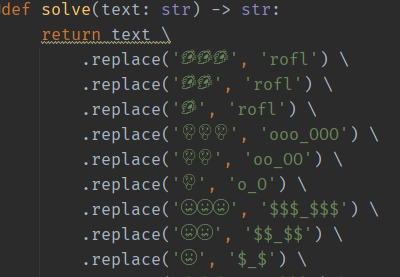
\includegraphics[width=7cm]{task6}
        \label{fig:solve6}
        \caption{Функция solve для задачи Emoji-Warrior}
    \end{figure}

    \subsection{Цветовод}
    \paragraph{}
    Решаем задачу как файловую.
    Скачиваем картинку в \verb|29.png|, открываем, смотрим цвет и инвертируем его.
    \begin{listing}[H]
        \begin{pythoncode}
def solve():
    img = Image.open('29.png')   # Открываем файл с изображением
    pix = img.load()             # Дооткрываем
    return '#' + \               # Возвращаем '#' + ...
           ''.join(              # ... соединенные пустой строкой элементы списка ...
               map(              # ... в котором применим функцию к каждому элементу списка ...
                   lambda colour: hex(255 - colour)[2:].upper().zfill(2),
                                 # Функция инвертирования цвета и преобразования к нужному виду
                   pix[0, 0]     # Список с данными о цветах пикселя по каналам
               )
           )
        \end{pythoncode}
        \label{lst:solve29}
        \caption{Функция solve для задачи Цветовод}
    \end{listing}

    \subsection{Кадровое агенство}
    \paragraph{}
    Для решения этой задачи желательно где-то раздобыть качественный список сотрудников школы.
    Отправляемся на сайт ШК, там в разделе \verb|Сведения об образовательной организации| есть ссылка на \verb|Руководство. Педагогический состав|.
    Переходим по ссылке, копируем список к себе в файл \verb|.csv| - простой формат для программной работы с таблицами:
    строки разделяются символами перевода строки (внезапно), а столбцы - запятыми.
    Важно заметить и исправть опечатку в отчестве Кирюшиной Натальи: на сайте пропущена буква А.
    \paragraph{}

    \begin{listing}[H]
        \begin{pythoncode}
staff = dict()                                            # Создаем пока пустой словарь
with open('14.csv') as file:                              # Открываем файл
    for line in file.readlines():                         # Читаем построчно
        man = line[:-1].split(',')                        # Получаем список с ФИО
        staff[' '.join([man[0], '...', man[2]])] = man[1] # Для строки Ф ... О ответ - Имя
        staff[' '.join([man[0], man[1], '...'])] = man[2] # Для строки Ф И ... ответ - Отчество

def solve(text):
    return staff[text]
        \end{pythoncode}
        \label{lst:solve14}
        \caption{Функция solve для задачи Кадровое агенство}
    \end{listing}

    \subsection{Вечеринка}
    \paragraph{}
    В этой задаче нужно принести печеньки с чаем.
    По понятным причинам, печенька - это файл cookie.
    По уже не таким понятным, но все еще достижимым причинам, чай - это содержимое файла.
    Так, вместе с авторизационными печеньками отправляем cookie с названием и значением \verb|tea|.
    На самом деле, достаточно и одного названия, или одного значения \verb|tea|.
    \begin{listing}[H]
        \begin{pythoncode}
def send_data():
    text = requests.post(
        host + 'tasks/task21',
        cookies={'login': login, 'token': token, 'tea': 'tea'})
    return text
        \end{pythoncode}
        \label{lst:solve21}
        \caption{Функция solve для задачи Вечеринка}
    \end{listing}

    \subsection{Календарь}
    \paragraph{}
    Решаем задачу как текстовую.
    Здесь нужно считать значение даты, добавить 701 один день и отправить обратно.
    Но ведь нужно считать все эти дни в месяце, високосные годы и другие сложные штуки.
    Но зачем, когда это уже сделано до нас?
    \paragraph{}
    Воспользуемся библиотекой \verb|datetime| для расчёта даты.
    \begin{listing}[H]
        \begin{pythoncode}
import datetime

def solve(text):
    days = datetime.datetime.strptime(text, '%d.%m.%Y') \ # Волшебный перенос строки
               .date().toordinal()                        # Получаем число дней с начала времён
    days += 701                                           # Добавляем 701 день
    return datetime.date.fromordinal(days) \              # Волшебный перенос строки
        .strftime('%d.%m.%Y')                             # Возвращаем значение даты
        \end{pythoncode}
        \label{lst:solve9}
        \caption{Функция solve для задачи Календарь}
    \end{listing}
    \paragraph{}
    Однако авторы задачи столкнулись с некоторой особенностью работы библиотеки под разными ОС.
    В некоторых случаях год в дате был написан без лидирующих нолей, то есть не обязательно четырьмя символами.
    % \newpage

    \subsection{Рукой подать}
    Скоро напишем разбор, но есть код решения без комментариев
    % TODO
    \begin{pythoncode}
class Vector():
    x: int
    y: int

    def __init__(self, x, y):
        self.x = x
        self.y = y

    def normalize(self):
        if self.x != 0: self.x = self.x // abs(self.x)
        if self.y != 0: self.y = self.y // abs(self.y)
    \end{pythoncode}

    \begin{pythoncode}
def solve():
    img = Image.open('43.png')
    pix = img.load()
    x1, y1, x2, y2 = None, None, None, None

    for x in range(img.size[0]):
        for y in range(img.size[1]):
            if pix[x, y] == (0, 0, 0):
                if x1 is None:
                    x1 = x
                    y1 = y
                else:
                    x2 = x
                    y2 = y
    vec = Vector(x2 - x1, y2 - y1)
    vec.normalize()

    if vec.x == 1 and vec.y == 1: x1 += 1; y1 += 1
    if vec.x == -1 and vec.y == 1: y1 += 1; x2 += 1
    if vec.x == 1 and vec.y == -1: x1 += 1; y2 += 1
    if vec.x == -1 and vec.y == -1: x2 += 1; y2 += 1

    if vec.x == 0 and vec.y == 1: y1 += 1
    if vec.x == 0 and vec.y == -1: y2 += 1
    if vec.y == 0 and vec.x == 1: x1 += 1
    if vec.y == 0 and vec.x == -1: x2 += 1

    length = ((x2 - x1) ** 2 + (y2 - y1) ** 2) ** 0.5

    round_len = round(length, 5)
    if int(length) != length:
        ans = str(round_len)
    else:
        ans = str(int(round_len))
    return ans
    \end{pythoncode}

    \subsection{CuSo4}
    \paragraph{}
    Решаем задачу как текстовую.
    \paragraph{}
    Для начала, используя информацию из условия, подготовим список химических элементов с номерами.
    Скопируем первые столбцы таблицы из Википедии в Excel, далее экспортируем (сохраняем как) \verb|.csv| -
    простой формат для программной работы с таблицами: строки разделяются символами перевода строки (внезапно),
    а столбцы - запятыми.
    Полученный файл сохраним как \verb|chemlist.csv|.
    \begin{listing}[H]
        \begin{pythoncode}
1,H
2,He
3,Li
4,Be
5,B
        \end{pythoncode}
        \caption{Фрагмент файла со списком химических элементов}
        \label{lst:chemlist}
    \end{listing}

    \paragraph{}
    Теперь необходимо в программе прочитать этот файл, после этого выполнить замены в правильном порядке.
    \begin{listing}[H]
        \begin{pythoncode}
with open('chemlist.txt', 'r') as chemlist:      # Открываем файл со списком элементов
    chem = [                                     # Создаем таблицу химических элементов
        i[:-1].lower().split(',')                # Разделяем строку на столбцы
        for i in chemlist.readlines()            # Из содержимого файла
    ]
chem.sort(key=lambda x: len(x[1]), reverse=True) # Сортируем по убыванию длины названия элемента

def solve(text):                                 # Объявляем функцию
    for elem in chem:                            # Для каждого химического элемента
        text = text.replace(elem[1], elem[0])    # Заменяем его название на номер
    return text                                  # Возвращаем текст
        \end{pythoncode}
        \caption{Функция solve для задачи CuSo4}
        \label{lst:solve23}
    \end{listing}

\end{document}